### Fourier transforms and convolutions

## Overview

In this chapter we will build on the concepts of Fourier analysis introduced in the last quarter. We will outline the theory of Fourier transforms and give examples of pairs of functions and their transforms. In the process, new theoretical constructs, such as the delta-function, will come into play. This will lead to the most important tool in the applications of Fourier transforms, convolution of two functions. I will give examples from imaging and crystallography, where Fourier transforms of data, described as  convolutions, are indispensable.

## Continuous Fourier Transform

### Fourier integral

So far we have only used the idea of frequency decomposition on functions which are either periodic (repeating) with period $L$, or equivalently, if we are only interested in the function over that interval. We may want to similarly analyze a continuous function which is not periodic, and in which we are interested over the whole real line. To achieve that, we generalize the notion of a Fourier series from a sum to an integral:

$$
G(f) =   \int_{-\infty}^\infty g(x) e^{i2\pi f x}dx; \; g(x) =  \int_{-\infty }^\infty G(f) e^{-i2\pi fx}df
$$

The first equation is called the *Fourier transform*, note that it changes the variable from $x$ (e.g. time or space) to $f$ (frequency). It is equivalent to the integral definition of $c_n$, except that $n$ was restricted to the integers, and $f$ can be any real number. This is why, for the second equation, defining the *Inverse Fourier transform*, the Fourier series becomes an integral: we have to add up the contributions of all real frequencies.

A note on notation: first, the signs of the frequencies in the definition of the Fourier series and the Fourier integral are reversed. I believe this is purely a matter of convention. Second, mathematicians prefer to define the Fourier transform and the inverse transform as follows:

$$
G(\omega) =   \int_{-\infty}^\infty g(x) e^{i \omega x}dx; \; g(x) =  \frac{1}{2\pi} \int_{-\infty }^\infty G(\omega) e^{-i\omega x}d\omega
$$

The difference between the two definitions is small, and conceptually can be distinguished by noting that the variable $f$ in the first definition refers to a pure frequency (times per unit of $x$) while the variable $\omega$ in the second definition refers to angular frequency (radians per unit of $x$). The textbook uses the second definition, but we will stick with the first, because it uses pure frequency $f$ and is more consistent with the definition of the Fourier series.

### Fourier transform examples

As we saw above, the units of the variables $x$ and $f$ are reciprocal to each other (e.g. second and 1/second, or meter and 1/meter), and although the functions $g(x)$ and $\widehat g(f)$ are in some sense the same function, they have an inverse relationship with each other. The Fourier transform and the inverse Fourier transform take functions between the two domains, and thus set up pairs of "inversely" related functions. In some cases, they are simply to compute and understand analytically. 

For instance, if we take the pure wave $\cos(2\pi x)$, it clearly contains only the frequencies $\pm 1$ (plus or minus because both positive and negative frequencies are inherent in any pure wave). You would expect its Fourier transform representation to be a double peak (symmetric about the origin) in the frequency space $f$, while everywhere else it is strictly zero. If we're dealing with Fourier series, of course, we just have two coefficients $c_1=1/2$ and $c_{N-1} = 1/2$, with all the others being zero. However, a single value has no weight on the real line (mathematically speaking, it has ``measure zero'', which means the same thing). So, mathematicians borrowed from physicists (Paul Dirac) the idea of an infinitely tall and infinitely thin spike which has finite area under the curve. This is called the delta function, and is written $\delta(x-a)$, where $a$ is the value at which it spikes. The Fourier transform of the pure cosine wave is then described as: 

$$ \frac{1}{2}\delta(f-1) + \frac{1}{2} \delta(f+1)$$

As a corollary, if we take the boring function $f(x)=1$, which can be thought of as a wave of zero frequency, its Fourier transform is given by simply $\delta(f)$ - that is, an infinite spike at frequency zero. Since $f(x)$ has an infinite mean and nothing else, this makes intuitive sense.

Conversely, the Fourier transform of a delta function $\delta(x-a)$ is given by:

$$ 
\int_{-\infty} ^\infty \delta(x-a) e^{i2\pi xf} dx = e^{i2\pi af} = \cos(2\pi af ) + i\sin(2\pi af)
$$

This uses the property of the delta function to ``pick out'' the value of the function it is integrated with, at the point matching its spike (in this case $a$). 

A function and its Fourier transformed counterpart are know as *Fourier pairs*. What we see is that functions which are widely distributed in one domain (like the constant function or the sines or cosines) have Fourier transforms which are infinitely thin, and vice versa. This a manifestation of the inverse property of the two domains, as we vaguely saw above. There is a general property of Fourier pairs that the wider a function, the narrower its Fourier counterpart. We have investigated the extremes, let us see where the happy medium lies. 

The Gaussian function $h(x)= e^{-ax^2}$ is a continuous bell-shaped curve which falls off sharply from its peak at zero, and has a finite area under the curve. It has the special property that its functional form is preserved by the Fourier transform: the Fourier partner of a Gaussian is also a Gaussian. Here is the verification:

$$
\int_{-\infty} ^\infty e^{-ax^2} e^{i2\pi xf} dx = \int_{-\infty} ^\infty e^{[-ax^2+i2\pi xf +\frac{\pi^2}{a}f^2] - \frac{\pi^2}{a}f^2}dx = e^{- \frac{\pi^2}{a}f^2} \int_{-\infty} ^\infty e^{-a(x-i\frac{\pi}{a}f)^2}dx = e^{- \frac{\pi^2}{a}f^2}  \sqrt\frac{\pi}{a}
$$

In the first step we did a trick called completing the square in the exponent, by adding the term $\pi/a f^2$ to make the first part of the expression be equal to $(\sqrt{a}x-i\frac{\pi}{\sqrt{a}}f)^2=a(x-i\frac{\pi}{a}f)^2$, and subtracting the same term. Then we split up the exponential into two factors, of which one ($e^{- \frac{\pi}{a}f^2}$)  is independent of the integration variable $x$, and can thus be brought out of the integral. What remains inside the integral is just a Gaussian function shifted over by a constant ($-i\frac{\sqrt\pi}{a}$). You can make a change of variables $y=x-i\frac{\sqrt\pi}{a}$, and because we are integrating over all values of $x$, the shift does not matter, the integral still contains all the area under the Gaussian curve. Finally, we know that the total area under a Gaussian $ e^{-ax^2}$ equals $\sqrt\frac{\pi}{a}$, hence the final step. 

Thus, the functions  $h(x)= e^{-ax^2}$  and $\widehat h(f) = \sqrt\frac{\pi}{a} e^{- \frac{\pi^2}{a}f^2}$ are a Fourier pair. If we choose $a = \pi$, you see that the exponentials of the two functions match, and the constant in $\widehat h(f)$ reduces to unity. The Gaussian function $ e^{-\pi x^2}$ is its own Fourier transform, not too wide, not too narrow - the Goldilocks function.

## Convolution and Fourier Transform

We now come to one more special property of the Fourier Transform which is useful in many different applications. The \emph{convolution} of two functions is defined as follows:

$$ h\circ g = \int _{-\infty} ^\infty h(x) g(y-x) dx $$ 

$g(y-x)$ is the function $g(y)$ horizontally translated by $x$. Thus, think about this integral as follows: for every number $y$, we sum over all the values of $h(x)$ multiplied by the value of $g(y-x)$, which is effectively shifted by $x$. 

Some important properties of the convolution, which can be easily shown by writing down the integral definition:
::: callout-note
## Properties of convolutions

*  convolution of two functions is commutative: $h  \circ  g = g  \circ h$
* convolution of two functions is associative: $ h\circ (g \circ f) = (h \circ g) \circ f$ 
* convolution of two functions is distributive: $h  \circ (g + f) = h  \circ f + h  \circ  f $
* convolution preserves shifts (translations): if $ f = h  \circ  g $, then $f(x-a) = h(x-a)  \circ  g = h  \circ  g (x-a)$
:::

### Examples
One simple example is based on the delta function $\delta(x-a)$ we saw in the previous lecture, which, if you recall picks out the value of the function it is integrated with that matches its spike at $a$. Thus, if we consider
$$ h(x)  \circ \delta(x-a) = \int _{-\infty} ^\infty h(x) \delta(y-x-a) dx = h(y-a) $$
That is, the delta function performed a shift, or repositioning of the function $h$ by its own peak position $a$. This property is often used in convolution applications, as we will see below. 

On the other extreme, we will consider a convolution with the opposite function: one which is infinitely wide. The convolution of a function with one which is unity everywhere, ($g(x) = 1$) results in the mean value of the function $h(x)$:

$$ h(x) \circ g(x) = \int _{-\infty} ^\infty h(x)  dx $$

### The Convolution Theorem
The reason why the convolution is so central to the application of Fourier Transforms is the following. The Fourier transform has the following special property with convolutions:
$$ \widehat{g \circ h} = \widehat {g} \widehat {h}$$

that is, the Fourier transform of a convolution of two function is the same as the product of the two separate FT. This enables a huge computational benefit for computing Fourier transforms of signals which are naturally convolved, because it is usually much easier to compute the FT of the two individual functions. 

There are many physical applications where convolutions arise naturally, for instance in communications, where one function can be thought of as a signal and the other the response, and the convolution given the observed communication. It is also invaluable in imaging, where one can get a repetition of different objects by defining one function to describe the object, and the other to describe the distribution of its locations. Convolution in this case gives the overall image with multiple objects, or with objects whose location is not precise, but has a smeared distribution. 


## Computational: Fourier transform in two dimensions, spectral analysis

### power spectrum in two dimensions
As we saw above, Fourier transforms can be computed exactly for some simple functions. In practice computational methods like the Fast Fourier Transform are used to find a numerical approximation of the Fourier transform. This means that only a discrete set of values of  $\widehat h(f)$ are computed. We will talk about this in the next lecture.

Here I want to focus on what we take away from Fourier transform analysis. Essentially, looking at $\widehat h(f)$ gives us a frequency-based representation of the original function  $h(x)$. We can see what types of frequencies are prevalent, which are absent, etc. To quantify this, however, we need to be more precise. The function  $\widehat h(f)$ is complex-valued, so we cannot even graph it in one dimension (Prove to yourself that: FT of an even function is purely real-valued, like the Gaussian example above, FT of an odd function is purely imaginary, and FT of mixed functions are complex, like the delta-function example above). Instead it is customary to consider the absolute value squared  $|\widehat h(f)|^2$, which is called the *power* of each frequency $f$.

This is convenient because the Parseval equality applies to Fourier integrals as  well:

$$ \int_{-\infty}^\infty |h(x)|^2 dx =  \int_{-\infty}^\infty |\widehat h(f)|^2 df $$

Therefore, we can look at the power distribution in frequency space (called the *power spectrum* as capturing an essential measure of the function $h(x)$ (its $L^2$ norm, if you want to get mathematical). This is the most common output of Fourier analysis, and the power spectrum plotted to describe how strong different frequencies are in the observed data.


### Application: analysis of time series data

One example of such application is the analysis of measurements recorded in time (called a *time series*, somewhat confusing for mathematicians since a series to them means a sum of multiple terms). For illustration, let us use the logistic iterated map that we studied in the first week: $x_{n+1} = rx_n(1-x_n)$. We will iterate it for several hundred steps (500 to be safe) to get it to converge to the attractor set, then record 500 steps of the steady-state time sequence and look at its power spectrum. Here is the time series and the power spectrum from $r=3.2$:
\begin{figure}[htbp] %  figure placement: here, top, bottom, or page
   \centering
   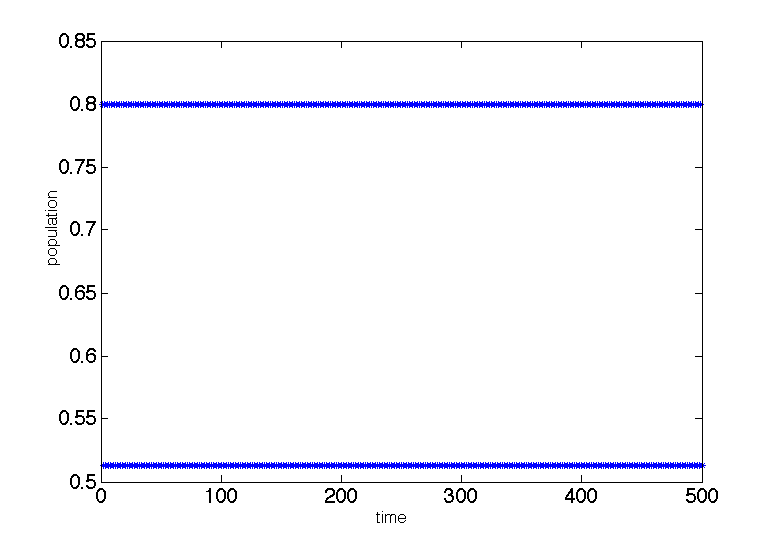
\includegraphics[width=3in]{log_seq_32.png}
   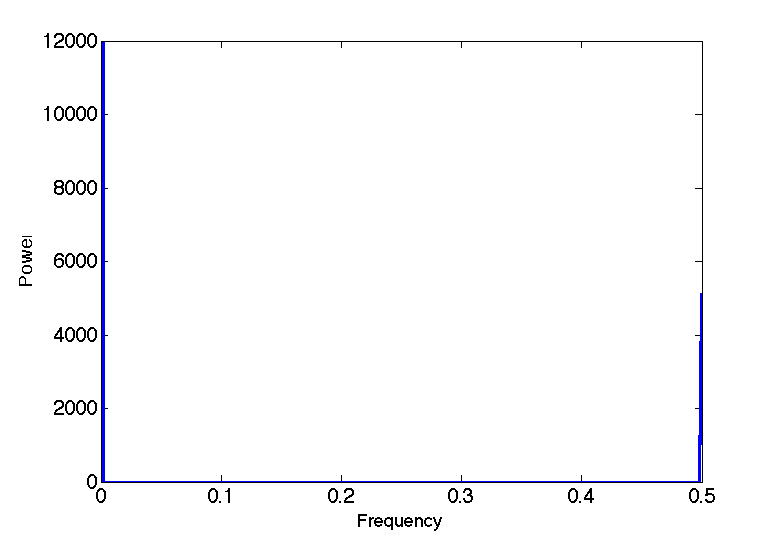
\includegraphics[width=3in]{log_pow_32.png}  
   \caption{The steady-state behavior of the logistic map for $r=3.2$: the sequence in time and its power spectrum.}
%   \label{fig:example}
\end{figure}
You can see that a period 2 oscillation is represented by two nonzero values in the power spectrum: zero frequency (sum of all values) and frequency 1/2 (period 2). This time of sharply peaked power spectrum is expected from 

Now let us take the value $r=3.8$, which leads to chaotic behavior, which is not periodic. The time series and the power spectrum are shown below:
\begin{figure}[htbp] %  figure placement: here, top, bottom, or page
   \centering
   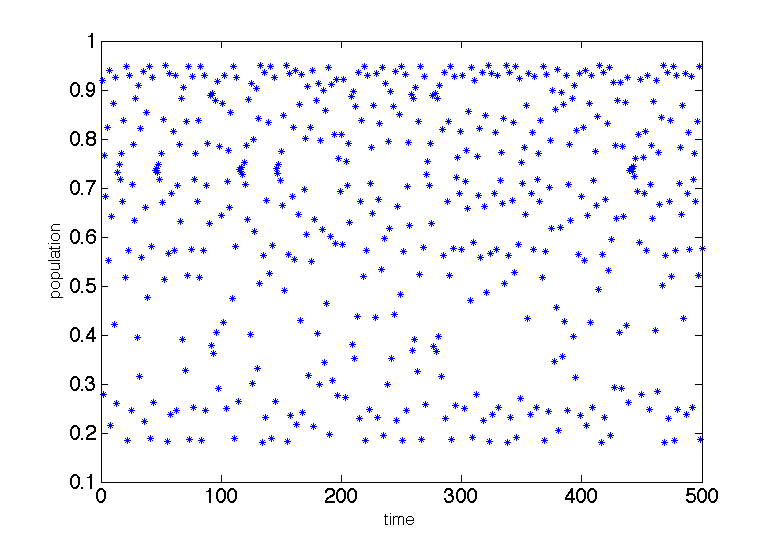
\includegraphics[width=3in]{log_seq_38.png}
   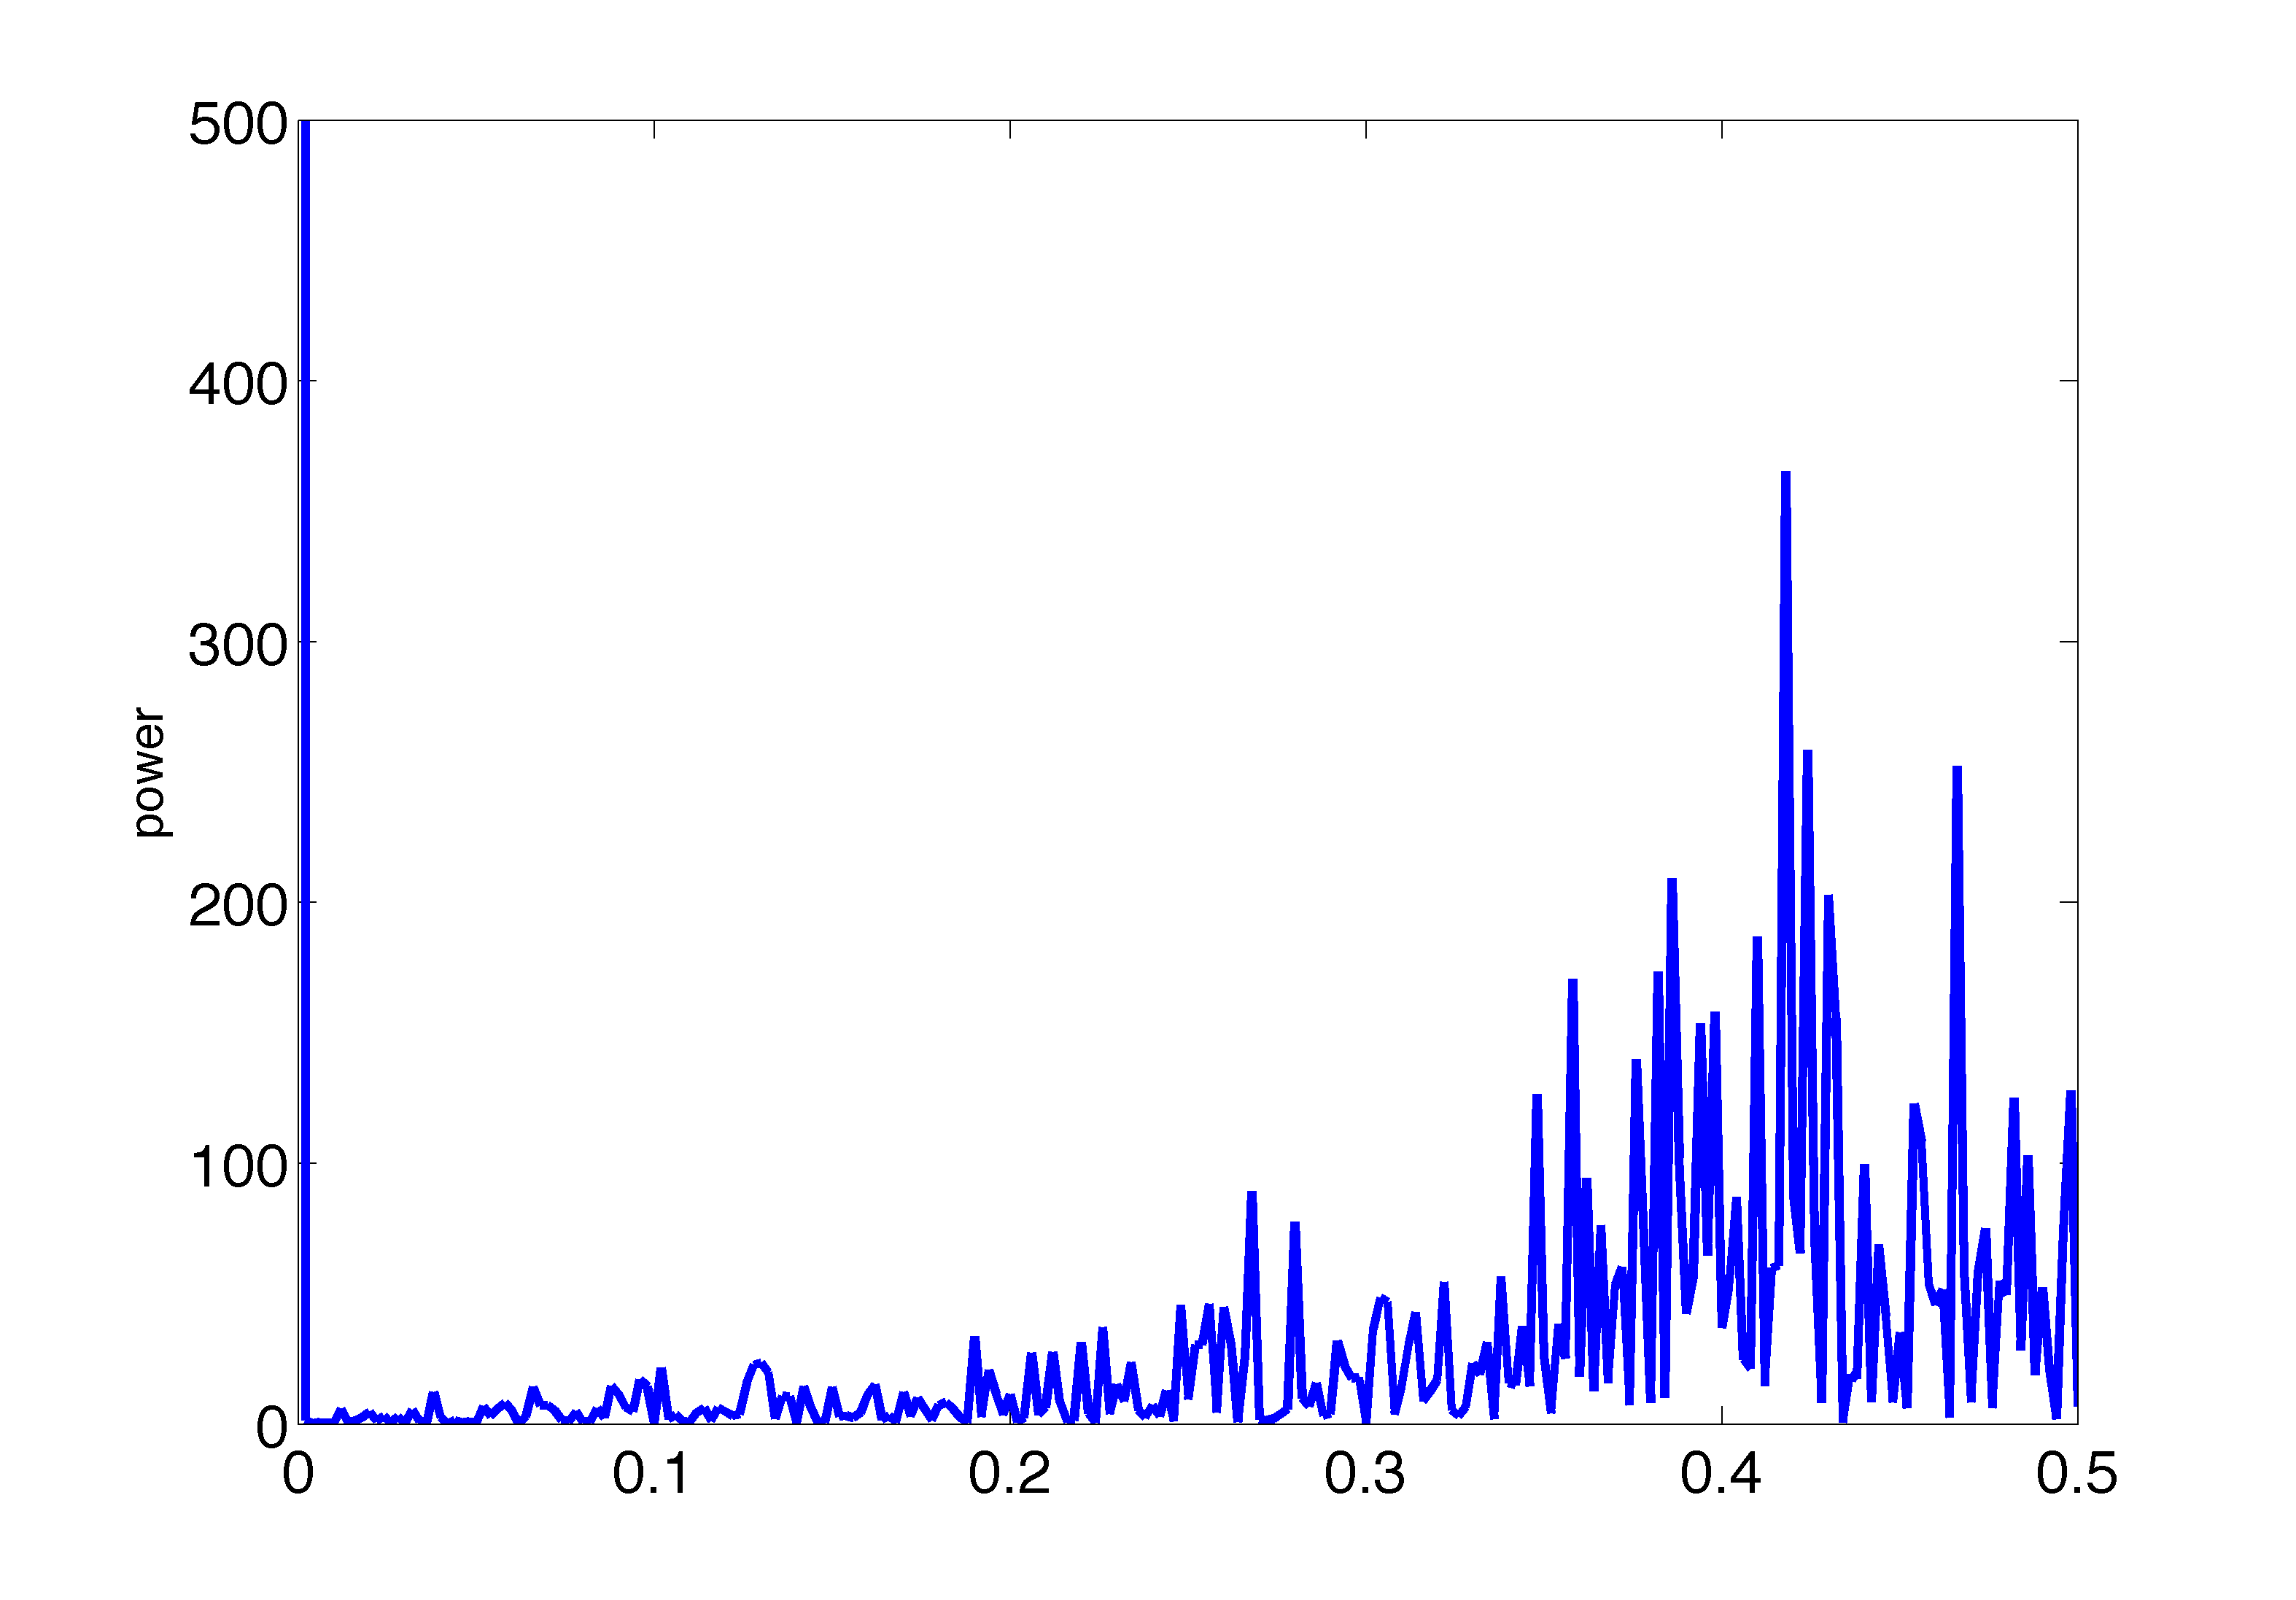
\includegraphics[width=3in]{log_pow_38.png}  
   \caption{The steady-state behavior of the logistic map for $r=3.8$: the sequence in time and its power spectrum.}
%   \label{fig:example}
\end{figure}
You can see that the power spectrum of a chaotic time series is dramatically different: all frequencies contribute, fast and slow, but the overall appearance of the power spectrum is ragged, as they are all represented with different powers. This is a tell-tale mark of chaos: lack of well-defined peaks, and an overall unstructured appearance.



## Synthesis: Fourier transform of crystal diffraction pattern
One important application of Fourier transforms is to optical scattering. Any time a light is scattered by an object, it results in a Fourier transform of the image of the object, and if enough photons are scattered, one can get a pretty complete picture. In the visible range, we can use lenses, such as in our eyes or in microscopes, to essentially perform the inverse Fourier transform. In X-ray crystallography, which is the primary tool for determining structures of biological molecules, it is not possible, because no optical lenses can interact with photons of that wavelength. We are left to perform the inverse Fourier transforms computationally.

Each atom in the crystal scatters photons with its electron cloud. While it is easy to describe the distribution of electrons in each atom, we have many atoms arranged in a lattice, each contributing to the diffraction intensity. If we consider them all, it will be a very difficult calculation. Instead, the convolution property allows us to find the Fourier transform of a single atom (a Gaussian function, so its Fourier pair is another Gaussian) and find the transform of the idealized lattice of points, both of which are easy calculations, and then multiply them together to find the Fourier transform of the whole lattice of atoms. This gives a simplified idea of how X-ray crystallographers can make sense out of a  diffraction pattern and re-create the electron density inside the molecules in the crystal. See {\tt http://www.mineralogie.uni-wuerzburg.de/crystal/teaching/conv\_a.html} for illustrations. 
